\documentclass[11pt,fleqn]{article}

\setlength {\topmargin} {-.15in}
\setlength {\textheight} {8.6in}

\usepackage{amsmath}
\usepackage{amssymb}
\usepackage{amsthm}
\usepackage{color}
\usepackage[utf8]{inputenc}
\usepackage{listings}
\usepackage{fullpage}
\usepackage{fancyvrb}
\usepackage{graphicx}

\graphicspath{ {./images/} }


\renewcommand{\labelenumii}{\theenumii.}

\newcommand{\mname}[1]{\mbox{\sf #1}}
\newcommand{\pnote}[1]{{\langle \text{#1} \rangle}}
\newcommand\todo[1]{\textcolor{red}{[TODO: #1]}}


\begin{document}

\begin{center}

  {\large \textbf{COMPSCI/SFWRENG 2C03}}\\[2mm]
  {\large \textbf{Data Structures and Algorithms}}\\[2mm]
  {\large \textbf{Ryszard Janicki}}\\[2mm]
  {\large \textbf{McMaster University}}\\[6mm]
  {\huge \textbf{Assignment 3}}\\[6mm]
  {\large \textbf{Name: Hishmat Salehi}}\\[2mm]
  {\large \textbf{MacId: Salehh6}}\\[2mm]
  {\large \textbf{Student number: 400172262}}\\[2mm]


\end{center}

\medskip

\begin{enumerate}
	\item 	
		\begin{enumerate}
			\item 
0: 5 $\rightarrow$ 2 $\rightarrow$ 6 \\
1: 4 $\rightarrow$ 8 $\rightarrow$ 11 \\
2: 5 $\rightarrow$ 6 $\rightarrow$ 0 $\rightarrow$ 3 \\
3: 10 $\rightarrow$ 6 $\rightarrow$ 2 \\
4: 1 $\rightarrow$ 8 \\
5: 0 $\rightarrow$ 10 $\rightarrow$ 2 \\
6: 2 $\rightarrow$ 3 $\rightarrow$ 0 \\
7: 8 $\rightarrow$ 11 \\
8: 1 $\rightarrow$ 11 $\rightarrow$ 7 $\rightarrow$ 4 \\
9: \\
10: 5 $\rightarrow$ 3 \\
11: 8 $\rightarrow$ 7 $\rightarrow$ 1
			\item Adjacency Matrix:

\begin{verbatim}
0, 0, 1, 0, 0, 1, 1, 0, 0, 0, 0, 0, 
0, 0, 0, 0, 1, 0, 0, 0, 1, 0, 0, 1, 
1, 0, 0, 1, 0, 1, 1, 0, 0, 0, 0, 0, 
0, 0, 1, 0, 0, 0, 1, 0, 0, 0, 1, 0, 
0, 1, 0, 0, 0, 0, 0, 0, 1, 0, 0, 0, 
1, 0, 1, 0, 0, 0, 0, 0, 0, 0, 1, 0, 
1, 0, 1, 1, 0, 0, 0, 0, 0, 0, 0, 0, 
0, 0, 0, 0, 0, 0, 0, 0, 1, 0, 0, 1, 
0, 1, 0, 0, 1, 0, 0, 1, 0, 0, 0, 1, 
0, 0, 0, 0, 0, 0, 0, 0, 0, 0, 0, 0, 
0, 0, 0, 1, 0, 1, 0, 0, 0, 0, 0, 0, 
0, 1, 0, 0, 0, 0, 0, 1, 1, 0, 0, 0, 
\end{verbatim}
		\end{enumerate}

\newpage

	\item $~$\\
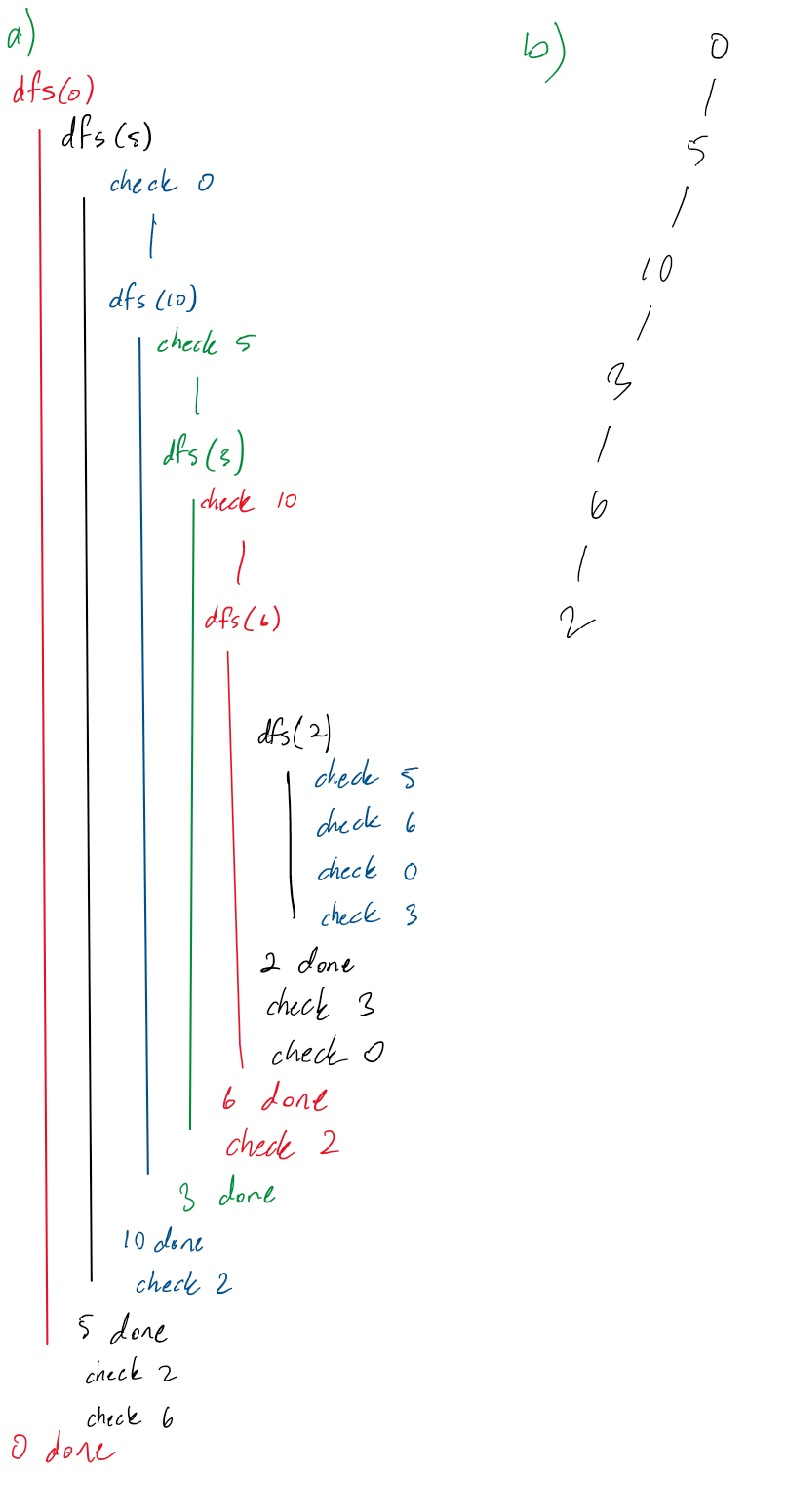
\includegraphics[scale=0.75]{Q2}

\newpage

	\item $~$\\
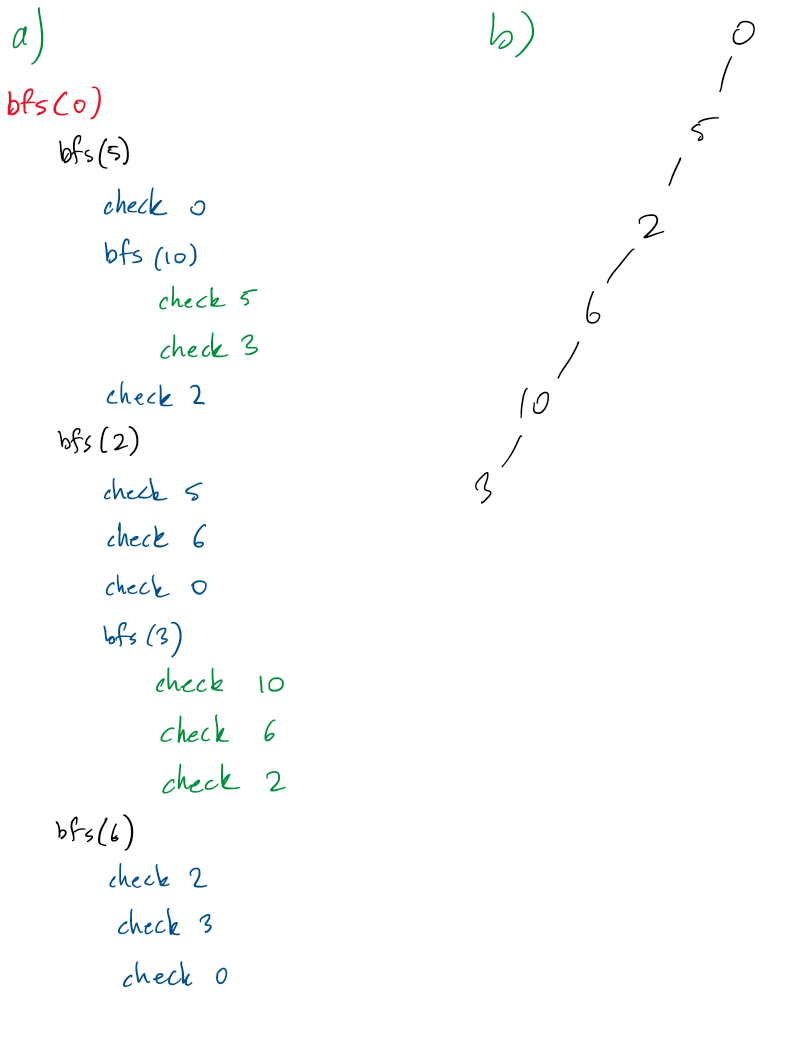
\includegraphics[scale=0.75]{Q3}
	\item Consider by contradiction that the edge of maximum weight in the cycle C, edge e, belongs to the MST of the graph.
Since MSTs do not contain cycles there is at least one edge in C that is not in the MST. Let's call one of these edges f.
Now add f to the MST. There is now a cycle in the MST. Since e has the maximum weight in the cycle C and all edge weights are distinct, it means that weight(f) < weight(e). 
Removing the edge e after having added the edge f would generate a new MST' with total weight less than the total weight in MST, contradicting its minimality.

\newpage

	\item 
		\begin{enumerate}
			\item
0: 6 $\rightarrow$ 5 \\
1: \\
2: 0 $\rightarrow$ 3 \\
3: 10 $\rightarrow$ 6 \\
4: 1 \\
5: 10 $\rightarrow$ 2 \\
6: 2 \\
7: 8 $\rightarrow$ 11 \\
8: 1 $\rightarrow$ 4 \\
9: \\
10: 3 \\
11: 8
			\item Adjacency Matrix:
\begin{verbatim}
0, 0, 0, 0, 0, 1, 1, 0, 0, 0, 0, 0, 
0, 0, 0, 0, 0, 0, 0, 0, 0, 0, 0, 0, 
1, 0, 0, 1, 0, 0, 0, 0, 0, 0, 0, 0, 
0, 0, 0, 0, 0, 0, 1, 0, 0, 0, 1, 0, 
0, 1, 0, 0, 0, 0, 0, 0, 0, 0, 0, 0, 
0, 0, 1, 0, 0, 0, 0, 0, 0, 0, 1, 0, 
0, 0, 1, 0, 0, 0, 0, 0, 0, 0, 0, 0, 
0, 0, 0, 0, 0, 0, 0, 0, 1, 0, 0, 1, 
0, 1, 0, 0, 1, 0, 0, 0, 0, 0, 0, 0, 
0, 0, 0, 0, 0, 0, 0, 0, 0, 0, 0, 0, 
0, 0, 0, 1, 0, 0, 0, 0, 0, 0, 0, 0, 
0, 0, 0, 0, 0, 0, 0, 0, 1, 0, 0, 0, 
\end{verbatim}
		\end{enumerate}
	\item \todo{Show steps pg. 589}
It's strongest component is 0 2 3 5 6 10.
	\item Topological order: \\
p $-$ n $-$ o $-$ s $-$ m $-$ r $-$ u $-$ y $-$ v $-$ w $-$ z $-$ q $-$ t $-$ x 

\newpage

	\item Suppose there are two minimum trees, A and B. Let e be the edge in just one of A,B with the smallest cost. 
Suppose it is in A but not B. Suppose e is the edge PQ. Then B must contain a path from P to Q which is not simply the edge e. 
So if we add e to B, then we get a cycle. If all the other edges in the cycle were in A, then A would contain a cycle, which it cannot. 
So the cycle must contain an edge f not in A. Hence, by the definition of e (and the fact that all edge-costs are different) the cost of f must be greater than the cost of e. 
So if we replace f by e we get a spanning tree with smaller total cost. Contradiction.
	\item 
	\begin{enumerate}
		\item Minimum spanning tree with Greedy Algorithm: \\
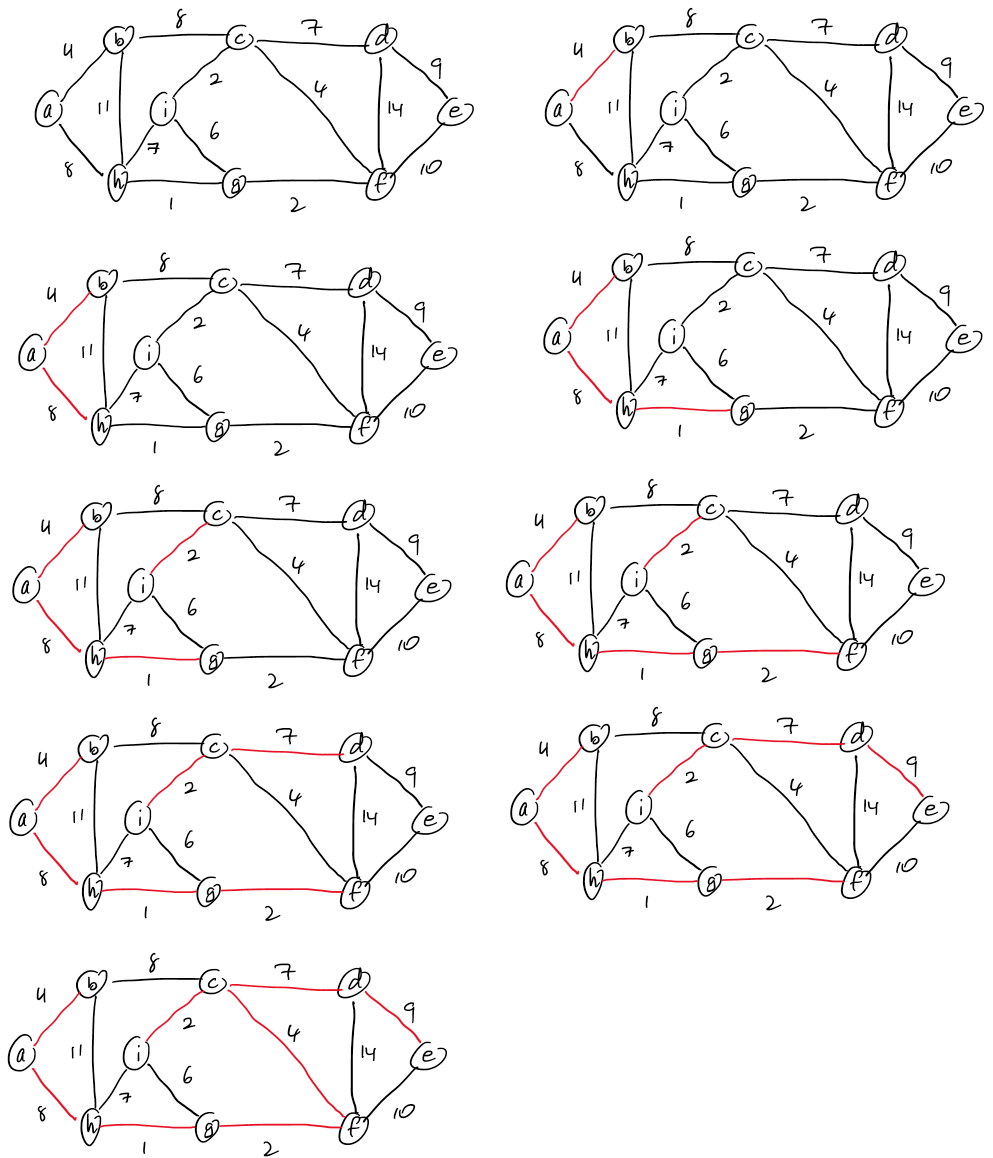
\includegraphics[scale=0.75]{Q9a}

\newpage

		\item Minimum spanning tree with Kruskal’s Algorithm: \\
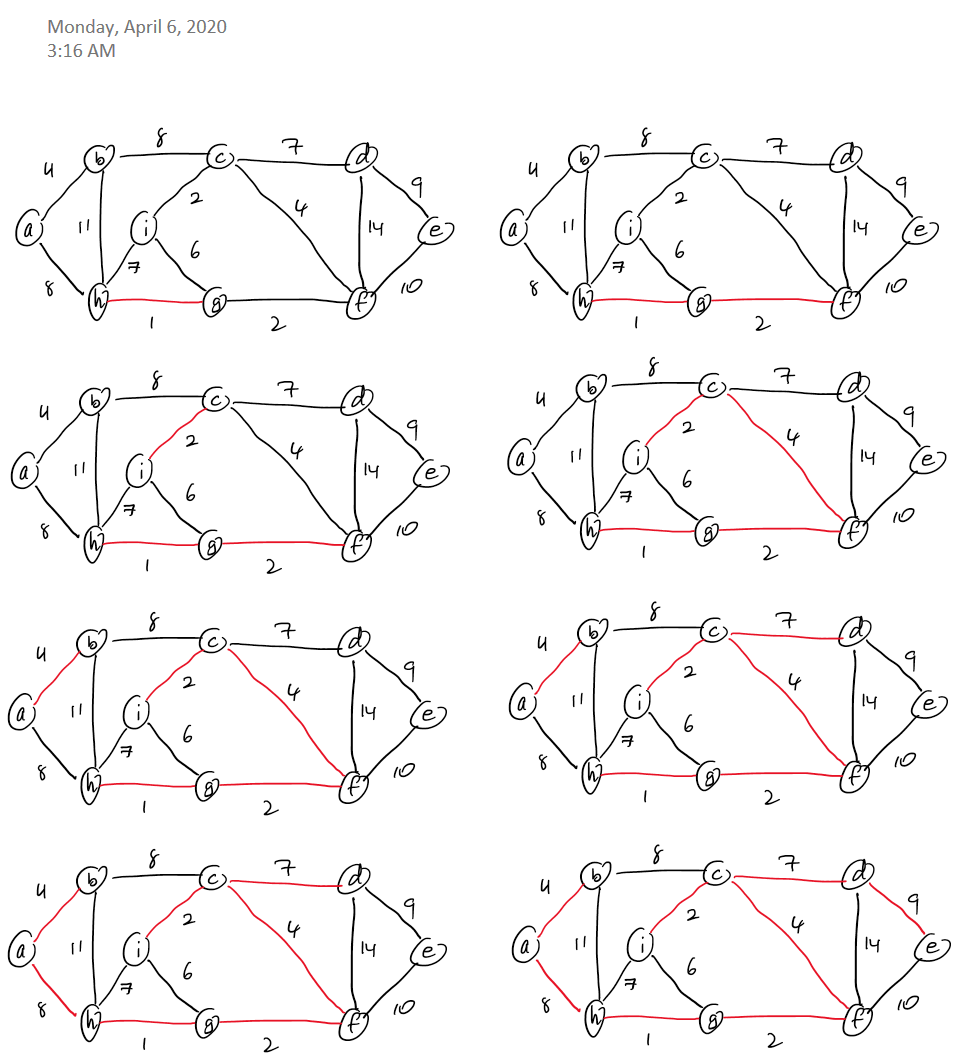
\includegraphics[scale=0.75]{Q9b}

\newpage

		\item Minimum spanning tree with Prim’s Algorithm: \\
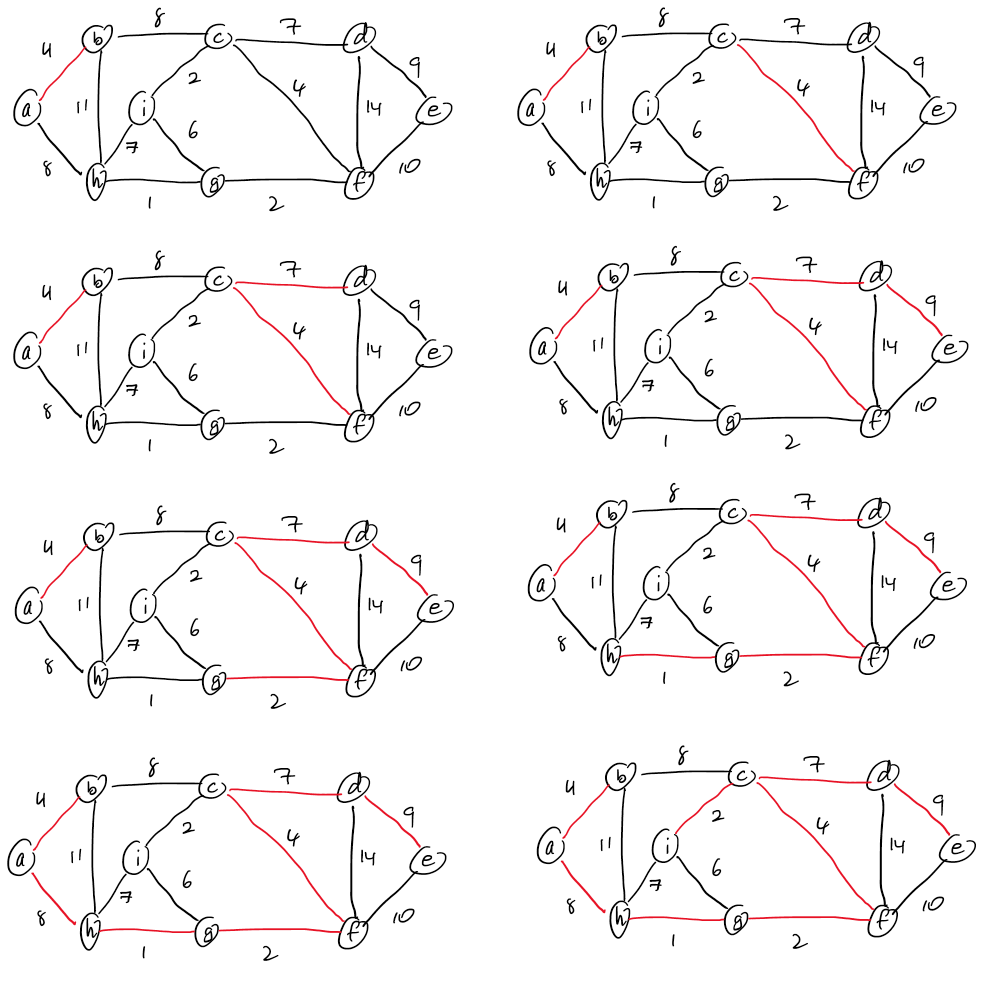
\includegraphics[scale=0.75]{Q9c}
	\end{enumerate}
	\item
a to a (0.00)  \\
a to b (2.00)  a$\rightarrow$b  2.00   \\
a to c (6.00)  a$\rightarrow$j  4.00   j$\rightarrow$c  2.00   \\
a to d (6.00)  a$\rightarrow$b  2.00   b$\rightarrow$f  3.00   f$\rightarrow$d  1.00   \\
a to e (8.00)  a$\rightarrow$l  5.00   l$\rightarrow$e  3.00   \\
a to f (5.00)  a$\rightarrow$b  2.00   b$\rightarrow$f  3.00   \\
a to h (5.00)  a$\rightarrow$h  5.00   \\
a to i (5.00)  a$\rightarrow$j  4.00   j$\rightarrow$i  1.00   \\
a to j (4.00)  a$\rightarrow$j  4.00   \\
a to k (7.00)  a$\rightarrow$b  2.00   b$\rightarrow$f  3.00   f$\rightarrow$d  1.00   d$\rightarrow$k  1.00   \\
a to l (5.00)  a$\rightarrow$l  5.00

	\item
s to s ( 0.00)  \\
s to t ( 2.00)  s$\rightarrow$y  7.00   y$\rightarrow$x -3.00   x$\rightarrow$t -2.00   \\
s to x ( 4.00)  s$\rightarrow$y  7.00   y$\rightarrow$x -3.00   \\
s to y ( 7.00)  s$\rightarrow$y  7.00   \\
s to z (-2.00)  s$\rightarrow$y  7.00   y$\rightarrow$x -3.00   x$\rightarrow$t -2.00   t$\rightarrow$z -4.00   \\

	\item 
\begin{Verbatim}
public double diameter(EdgeWeightedDigraph edgeWeightedDigraph) {
	double diameter = Double.NEGATIVE_INFINITY;

	for (int v = 0; v < edgeWeightedDigraph.V(); v++) {
		DijkstraSP dijkstraSP = new DijkstraSP(edgeWeightedDigraph, v);

		for (int v2 = 0; v2 < edgeWeightedDigraph.V(); v2++) {
			if (dijkstraSP.distTo(v2) > diameter) {
				diameter = dijkstraSP.distTo(v2);
			}
		}
	}

	return diameter;
}
\end{Verbatim}

	\item
r to r (0.00)  
r to s (5.00)  r->s  5.00   
r to t (3.00)  r->t  3.00   
r to x (10.00)  r->t  3.00   t->x  7.00   
r to y (7.00)  r->t  3.00   t->y  4.00   
r to z (5.00)  r->t  3.00   t->z  2.00

	\item

\end{enumerate}

\end{document}


